%==============================================================
% BAB I  PENDAHULUAN
%==============================================================

\chapter{PENDAHULUAN}

%--------------------------------------------------------------
\section{Latar Belakang}
%--------------------------------------------------------------

Deforestasi adalah perubahan fungsi hutan menjadi penggunaan lahan lain, terlepas dari apakah hal itu disebabkan oleh manusia atau tidak \citep{FAO2023}. Konversi hutan tropis menjadi perkebunan monokultur telah berlangsung secara masif selama dua dekade terakhir. Dari 2002 sampai 2024, Kalimantan Barat kehilangan 1.4 Mha hutan primer basah, menyumbang 33\% dari total kehilangan tutupan pohon dalam periode yang sama. Area total hutan primer basah di Kalimantan Barat berkurang 20\% dalam periode waktu ini \citep{GFW2026}.

Deteksi perubahan pada citra satelit adalah tugas utama dalam \textit{remote sensing} yang tak hanya dapat diaplikasikan dalam kasus pemantauan lingkungan, namun juga pada kasus lain seperti penilaian bencana dan perencanaan perkotaan. Metode \textit{pixel-based} tradisional seperti diferensiasi citra, pembandingan, dan regresi hanya bersandar kepada perbandingan spektral atau intensitas \citep{richards2022remote}. Walaupun secara komputasi lebih efisien, pendekatan tradisional rentan terhadap noise, variasi pencahayaan, dan ketidakselarasan geometrik sehingga membatasi ketahanan pada kondisi nyata \citep{Ali2026,richards2022remote}.

\textit{Deep Learning} (DL) telah berkembang dan berhasil merevolusi bidang ini dengan memungkinkan pembelajaran fitur secara otomatis. \textit{TransSiamUNet}, sebuah arsitektur DL yang mengombinasikan \textit{Siamese networks}, \textit{U-Net segmentation}, dan \textit{Vision Transformers} (ViT) berhasil mendeteksi perubahan pada dataset LEVIR-CD dengan \textit{F-1-score} 0,928 \citep{Ali2026}. 

Meskipun menunjukkan hasil yang menjanjikan, arsitektur \textit{TransSiamUNet} memiliki kompleksitas tinggi dan membutuhkan sumber daya yang besar, sehingga kurang efisien untuk implementasi pada kasus yang mengharuskan keterbatasan sumber daya. Selain itu, model DL memiliki kecenderungan bersifat \textit{black box}, sehingga sulit untuk memahami proses inferensi model. Kurangnya interpretabilitas dapat menurunkan tingkat kepercayaan serta menghambat penerapan pada aplikasi kritis seperti pemantauan lingkungan.

Oleh karena itu, penelitian ini mengusulkan pendekatan berbasis DL untuk mendeteksi perubahan deforestasi di Kalimantan menggunakan citra satelit multispektral. Secara khusus, penelitian ini berfokus pada pengembangan arsitektur \textit{Siamese U-Net} yang dimodifikasi untuk mencapai keseimbangan antara performa dan efisiensi, serta mengintegrasikan teknik \textit{Explainable Artificial Intelligence} (XAI) guna meningkatkan interpretabilitas model. 


%--------------------------------------------------------------
\section{Rumusan Masalah}
%--------------------------------------------------------------

\begin{enumerate}
    \item Bagaimana performa model \textit{deep learning} (Siamese U-Net) dalam mendeteksi perubahan deforestasi pada citra multispektral Sentinel-2 di Kalimantan?
    \item Apakah modifikasi arsitektur Siamese U-Net dapat meningkatkan performa deteksi perubahan dibandingkan model baseline?
    \item Bagaimana \textit{Explainable Artificial Intelligence} (Grad-CAM) dapat digunakan untuk menginterpretasikan hasil deteksi perubahan?
\end{enumerate}


%--------------------------------------------------------------
\section{Tujuan}
%--------------------------------------------------------------

\begin{enumerate}
    \item Mengimplementasikan dan mengevaluasi model Siamese U-Net untuk deteksi perubahan deforestasi.
    \item Mengembangkan modifikasi arsitektur untuk meningkatkan performa model berdasarkan teknik evaluasi \textit{Intersection over Union} (IoU) dan \textit{F-1-Score}.
    \item Menganalisis interpretabilitas model menggunakan metode \textit{Explainable Artificial Intelligence} (Grad-CAM).
\end{enumerate}

%--------------------------------------------------------------
% CONTOH GAMBAR
% - Gambar ditempatkan dengan [H] atau [htbp]
% - Caption: di bawah gambar, format "Gambar N Judul"
% - Tanpa bold, tanpa titik dua, hanging indent otomatis
%--------------------------------------------------------------

% commented
\begin{comment}
\begin{figure}[H]
  \centering
  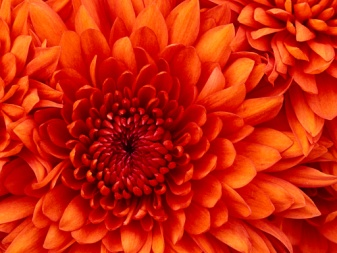
\includegraphics[width=0.5\textwidth]{images/contoh_gambar1}
  \caption{Contoh gambar}
  \label{fig:contoh_gambar1}
\end{figure}
\end{comment}

%--------------------------------------------------------------
\section{Manfaat}
%--------------------------------------------------------------

\begin{enumerate}
    \item Memberikan kontribusi dalam pengembangan metode \textit{deep learning} untuk deteksi perubahan tutupan lahan berbasis citra multispektral, khususnya melalui eksplorasi arsitektur \textit{Siamese U-Net} dan pendekatan \textit{Explainable AI}.

    \item Menyediakan pendekatan yang dapat digunakan untuk mendukung pemantauan deforestasi secara lebih efisien dan terotomatisasi.
\end{enumerate}


%--------------------------------------------------------------
% CONTOH TABEL
% Panduan tabel IPB:
% - Caption selalu di atas tabel
% - Format "Tabel N Judul tabel" (tanpa titik dua, tanpa bold)
% - Hanging indent: baris lanjutan rata dengan awal judul
% - Gaya three-line: \toprule, \midrule, \bottomrule (booktabs)
% - Tidak ada garis vertikal
% - Tidak ada garis horizontal internal kecuali setelah header
% - Catatan kaki tabel menggunakan notasi superskrip huruf kecil
%   dan ditulis di bawah tabel dengan \tabularnote atau manual
%--------------------------------------------------------------

\begin{comment}
\begin{table}[htbp]
  \caption{Tingkat kekerasan dan kandungan gula buah pisang ambon
           pada suhu simpan yang berbeda dan pemberian putresina}
  \label{tab:pisang_ambon}
  \centering
  \small  % Tabel ukuran agak lebih kecil jika konten padat
  \begin{tabular}{lcccccc}
    \toprule
    \multirow{2}{*}{Perlakuan}
      & \multicolumn{6}{c}{Kekerasan buah dan kandungan gula pada hari ke-} \\
    \cmidrule(lr){2-7}
      & \multicolumn{2}{c}{0} & \multicolumn{2}{c}{7} & \multicolumn{2}{c}{14} \\
    \cmidrule(lr){2-3}\cmidrule(lr){4-5}\cmidrule(lr){6-7}
      & Keras$^{\,\mathrm{a}}$ & Gula & Keras$^{\,\mathrm{a}}$ & Gula
      & Keras$^{\,\mathrm{a}}$ & Gula \\
    \midrule
    \multicolumn{7}{l}{\textit{Suhu simpan}} \\
    \quad 15 ºC  & 10.20a & 0.38a & 13.40a & 0.56a & 11.83a & 0.73a \\
    \quad 28 ºC  & 10.64a & 0.55a & 14.22a & 1.82a & 88.43b & 14.41b \\
    \multicolumn{7}{l}{\textit{Putresina}} \\
    \quad Dengan putresina  & 11.07a & 0.53a & 13.23a & 0.87a & 21.19a & 6.98a \\
    \quad Tanpa putresina   & 10.76a & 0.40a & 14.40a & 1.52a & 41.82b & 6.91a \\
    \bottomrule
  \end{tabular}
  % Catatan kaki tabel: rata kiri, ukuran normal, di bawah garis bawah
  \begin{minipage}{\linewidth}
    \vspace{2pt}
    \footnotesize
    $^{\mathrm{a}}$Angka-angka pada kolom yang sama yang diikuti oleh huruf yang
    sama tidak berbeda nyata pada taraf uji 5\% (uji selang berganda Duncan).
  \end{minipage}
\end{table}
\end{comment}

%--------------------------------------------------------------
\section{Ruang Lingkup }
%--------------------------------------------------------------

\begin{enumerate}
    \item Penelitian difokuskan pada deteksi perubahan deforestasi menggunakan citra satelit multispektral.

    \item Wilayah studi dibatasi pada Kalimantan sebagai studi kasus.

    \item Data yang digunakan adalah citra Sentinel-2 Level-2A dan label dari Hansen Global Forest Change.

    \item Pendekatan yang digunakan terbatas pada model \textit{deep learning} berbasis U-Net, khususnya \textit{Siamese U-Net} dan variasi modifikasinya.

    \item Tahapan penelitian mencakup pra-pemrosesan data, pelatihan model, dan evaluasi performa menggunakan metrik seperti IoU dan F1-score.

    \item Analisis interpretabilitas dilakukan menggunakan metode \textit{Explainable Artificial Intelligence} (\textit{Grad-CAM}).

    \item Penelitian ini tidak mencakup pengembangan sistem produksi berskala besar, dan visualisasi hasil dilakukan secara terbatas untuk keperluan analisis.
\end{enumerate}

\begin{comment}
Bagian ini menjelaskan batasan dan ruang lingkup penelitian yang dilakukan
agar pembaca dapat memahami cakupan serta keterbatasan studi.

% Contoh gambar dengan judul panjang lebih dari satu baris.
% Baris kedua otomatis dimulai tepat di bawah huruf pertama judul (hanging indent).

\begin{figure}[H]
  \centering
  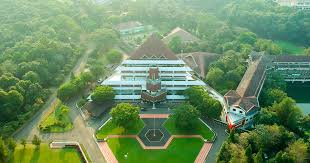
\includegraphics[width=0.7\textwidth]{images/contoh_gambar2}
  \caption{Contoh judul gambar lebih dari satu baris maka baris kedua
           dimulai tepat di bawah huruf pertama judul gambar}
  \label{fig:contoh_gambar2}
\end{figure}
\end{comment}

%--------------------------------------------------------------

\section{Hipotesis}
%--------------------------------------------------------------

\begin{enumerate}
    \item Model \textit{Siamese U-Net} mampu mendeteksi perubahan deforestasi pada citra multispektral Sentinel-2 dengan performa yang baik.

    \item Modifikasi arsitektur \textit{Siamese U-Net} dapat meningkatkan performa deteksi perubahan dibandingkan model baseline.

    \item Pendekatan \textit{Explainable AI} (\textit{Grad-CAM}) mampu memberikan interpretasi yang relevan terhadap hasil prediksi model.
\end{enumerate}
